\documentclass[a4paper,12pt,oneside,titlepage]{article} 
\usepackage[T1]{fontenc}
\usepackage[english]{babel}
\usepackage[utf8]{inputenc}
\usepackage{amsfonts} 
\usepackage{amssymb}
\usepackage{amsthm}
\usepackage{amsmath}
\usepackage{graphicx}
\usepackage{array}
\usepackage{booktabs}
\usepackage{siunitx}
\sisetup{output-decimal-marker={.}}
\usepackage{bm}
\usepackage{mathrsfs}
\usepackage[numbers]{natbib}
\usepackage{epstopdf}
\usepackage{subfig}
%\usepackage{subfloat}
\usepackage{multirow}
\usepackage{bm}
\usepackage{float}

\usepackage{verbatim}
\usepackage{hyperref}
\hypersetup{
	colorlinks=true,
	linkcolor=black,
	filecolor=magenta,      
	urlcolor=black,
}
\usepackage{caption}
\graphicspath{{images/}}            %path image
\captionsetup{tableposition=top,figureposition=bottom,format=hang, font=scriptsize}
\usepackage[skip=2pt]{caption}
\usepackage{cleveref}

%\captionsetup{format=myformat}

%\documentclass[paper=a4]{scrartcl}
\usepackage[utf8]{inputenc}
\usepackage[T1]{fontenc}
\usepackage[section]{placeins}
%\usepackage[showframe]{geometry}
%\usepackage{layout}
\setlength{\voffset}{0in}
%\setlength{\headsep}{5pt}
%\textwidth{600}
%\usepackage[a4paper]{geometry}
\usepackage{calc}
\usepackage[textheight=50\baselineskip+10pt]{geometry}

\begin{document}
	
	\thispagestyle{empty}
	\setcounter{page}{0}
	
	\begin{center}
		\huge
		POLITECNICO DI TORINO\\[1.cm]
		\Large
		ICT for Health \\
		\vspace{0.5cm}
		\Large
		Report Laboratory 1\\[1.3cm]
		
		\vspace{0.5cm}
		
\includegraphics[scale=2]{logo.jpg}
	\end{center}
	\vspace{1.cm}
	
	\begin{flushleft}
		\Large
		\noindent {\bfseries Professor:}\\
		Monica Visintin\\[0.2cm]
	\end{flushleft}
	\vspace{1cm}
	
	
	\begin{flushright} 
		\Large
		\noindent{\textbf{Student}:}\\
		Iman Ebrahimi Mehr S250190\\[0.2cm]
	\end{flushright} 
	\vspace{2cm}
	\begin{center}
		\Large
		A.Y.2019-2020
	\end{center}
	
	\newpage
	\thispagestyle{empty}
	\tableofcontents
	
	
	\newpage
	\section{Introduction}
	\subsection{\textbf{Parkinson’s disease (PD)}}
	\textbf{Parkinson’s disease (PD)} is the most common age-related motoric neurodegenerative disease initially described in the 1800’s by James Parkinson as the ‘Shaking Palsy’; Motor symptoms in PD are tightly linked to the degeneration of substantia nigra dopaminergic neurons and their projections into the striatum; also it’s characterized by resting tremor, rigidity, akinesia and bradykinesia. The sick neurons project to other structures in the basal ganglia causing the loss of function of the latter that is involved in the coordination of the body movement.
	
	\textbf{Unified Parkinson’s Disease Rating Scale (UPDRS)} is a worldwide scale used to evaluate the progression of the disease. The UPDRS is composed of four sub-scales and each of them contain some items (42 in total), which assess impairment related to the PD. The subclass are : 
	\begin{itemize}
		\item mentation, behavior and mood (composed of 4 items)
		\item activities of daily living (composed of 13 items)
		\item motor (composed of 14 items)
		\item complication of therapy (composed of 11 item)
	\end{itemize}
	More in particular, the speech symptoms related to Parkinson’s Disease are: overall loudness level is reduced; rate of speech becomes too slow or too fast; difficulty initiating speech or inappropriate pauses; voice is tremulous and monotonous; hoarse/breathy vocal quality; articulatory effort is reduced or imprecise.
	
	\subsection{Goal of laboratory}
	The goal of laboratory is to find a linear correlation, whether exist or not, between the features of the patients and the grade of the UPDRS, using linear regression. The regression can be realized through different methods or algorithms where each of them starts from a set of observed values (dependent variable) $y(n)  \varepsilon R$, with $n = 1, ..,N$ , also called regressand, and goes back to the independent variable $x(n)  \varepsilon R^{N}$, also called regressor. In linear regression we assume that
	\begin{equation}
	y(n) = [x (n)]^T w + v(n) = Xw + v(n)
	\end{equation}
	where $w = [w_{1}, ..,w_{F}]$ is a set of weight to be found (they represent the correlation between the regressor and the regressand) and $v(n)$ is the error.
	Now by defining the \textbf{cost function} as $f(w) = ||y-Xw||^2$ which we want to minimize it because by minimizing this, we get $v(n) = 0$ and so $y = Xw$. This means that, knowing the values of w and $X$ , we can predict the values of y. To summarize, we’re going to find an optimum set of weights $w^*$ which allow us to find a feature $y(n)$ by a given set of other features stored in a matrix $X$.
	
	\newpage
	\section{The data}
	\subsection{The data set}
	The dataset which we’re going to use in this laboratory was created by the University of Oxford from 42 people recruited in six-month trial of a telemonitoring device for remote symptom progressing monitoring. These data are stored into a table which is composed of 26 columns and 5875 rows. Each column represent a useful feature to describe the severity of the PD, for example there is stored patience number, age, gender, time interval from baseline recruitment date, motor UPDRS, total UPDRS and other 16 voice measurements. Each row corresponds to a single measurement of each feature on a given patient.
	\subsection{Preprocessing}
	First of all we want to standardize our data which help us to build features that have similar ranges to each other and make them comparable, to do this procedure we arround our data by Mean of data and divide them to Standard Deviation as follow:
	\begin{equation}
	z = \frac {x - \mu}{\delta}
	\end{equation}
	In the next step we divided our data into 3 part as:
	\begin{itemize}
		\item \textbf{training dataset}: used to train algorithms and to evaluate if they are correct or not. The result of executing algorithms is the set of weights $w^*$;
		\item \textbf{validation dataset}: used in some algorithms to optimize it by changing some given parameters (like the number of iterations in iterative algorithm) and to adjust the $w^*$;
		\item \textbf{testing dataset}: used finally to predict the y(n) with the w* and calculate error of algorithms.
	\end{itemize}
	
	
	\section{Methods and Algorithms}
		
	\subsection{LLS pseudoinverse}
	Starting from the equation of the linear regression $y(n) = Xw + v(n)$ , the Linear Least Square (LLS) algorithm try to find the w that minimizes the cost function $f(w) = ||y-Xw||^2$ that can be written as
	\begin{equation}
	f(w) =[y-Xw]^T [y-Xw] = y^Ty - y^TXw - w^TX^Ty + w^TX^TXw
	\end{equation}
	Now, we evaluate the gradient (multi-variable generalization of the derivative) and set it equal to 0.
	\begin{equation}
	\nabla(w) =-2X^Ty+2X^TXw = 0
	\end{equation}
	And finally by simplifying we get the optimum weight vector as:
	\begin{equation}
	w^*= [X^TX]^{-1}X^Ty
	\end{equation}
	The term: $[X^TX]^{-1}X^T$ is the pseudoinverse of the rectangular matrix X (train data).
	\subsubsection{Result}
	The optimum values of $W^*$ are shown in figure \ref{fig:lls_a}. To evaluate the algorithm we compare the real vector $y$ , extracted from the training and testing dataset, with the predicted vector $\hat {y} = Xw^*$, calculated by executing the
	algorithm, as we can see in figures \ref{fig:lls_c} and \ref{fig:lls_d}.\\
	The figure \ref{fig:lls_b} represent the relation between the error, which is the difference $y-\hat {y}$,
	and number of times it occurs. The histogram has been realized by using training dataset(blue) as well as testing dataset(orange).
	\begin{figure}[H]
		\centering
		\begin{center}			
			\subfloat[][\emph{$w^*$ optimize vector}\label{fig:lls_a}]
			{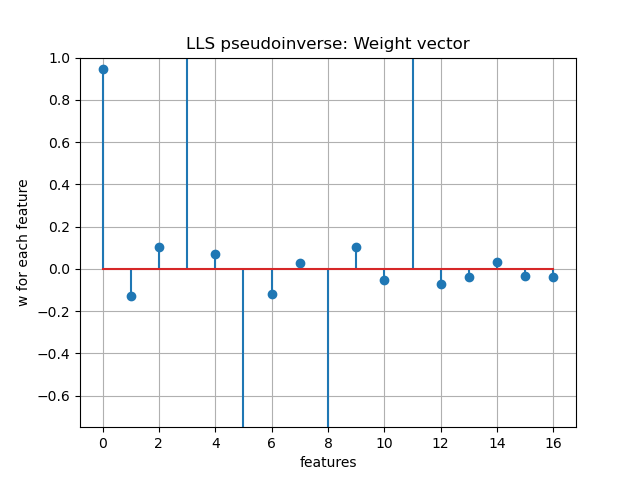
\includegraphics[width=.5\textwidth]{LLSpseudoinverseWeightvector.PNG}}
			\subfloat[][\emph{$\hat {y} - y$ for Test and train}\label{fig:lls_b}]
			{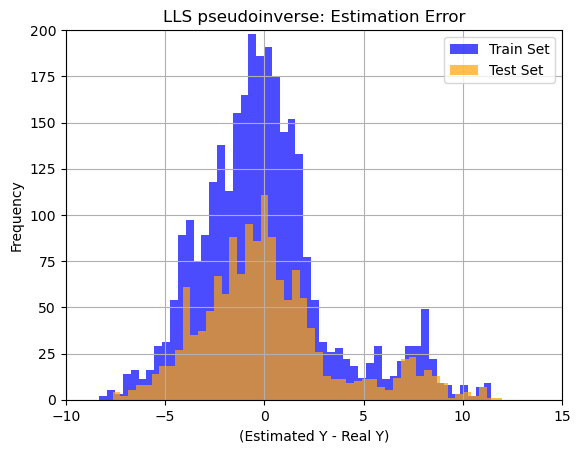
\includegraphics[width=.5\textwidth]{LLSpseudoinverseEstimationError_test.PNG}}\\
			\subfloat[][\emph{$\hat { \mathbf { y } } _ { \mathrm { train } } \textit{{\scriptsize VS} }  \mathbf {y } _ { \mathrm { train } }$}\label{fig:lls_c}]
			{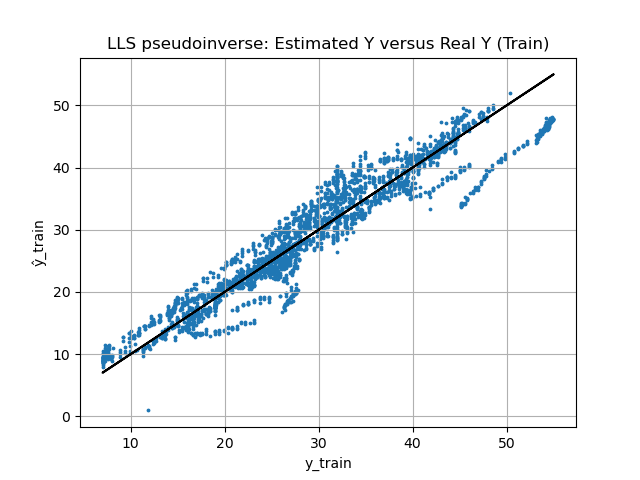
\includegraphics[width=.5\textwidth]{LLSpseudoinverseEstimatedYversusRealY_train.PNG}}
			\subfloat[][\emph{$\hat { \mathbf { y } } _ { \mathrm { test } } \textit{{\scriptsize VS} }  \mathbf {y } _ { \mathrm { test } }$}\label{fig:lls_d}]
			{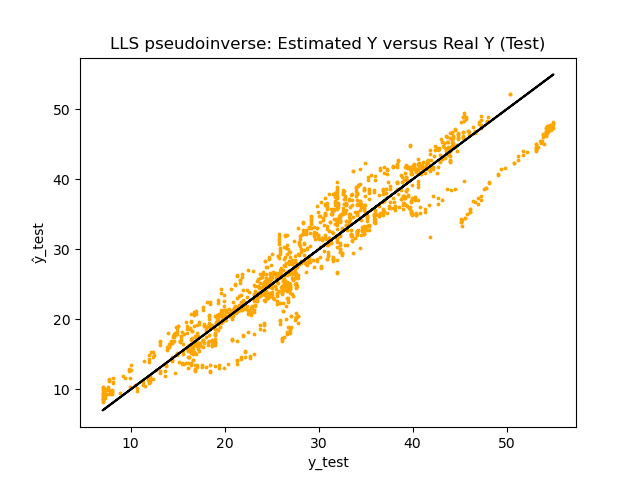
\includegraphics[width=.5\textwidth]{LLSpseudoinverseEstimatedYversusRealY_test.PNG}}\\
			\caption{Linear Least Square}
			\label{fig:lls}
		\end{center}
	\end{figure}
	
	
	
	\subsection{The gradient algorithm}
	It is a first-order optimization algorithm. This means it only takes into account the first derivative when performing the updates on the parameters. On each iteration, we update the parameters in the opposite direction of the gradient of the objective function $f(w)$. The size of the step we take on each iteration to reach the local minimum is determined by the learning rate $\gamma$. 
	After having evaluated the gradient as:
	\begin{equation}
	\nabla f ( \mathbf { w } ) = 2 \mathbf { X } ^ { \top } ( \mathbf { X w } - \mathbf { y } )
	\end{equation}
	Starting from an initial guess $w_{i}$  with $i=0$ and being $\gamma$ a positive constant which we call it step size, we find the new point as:
	\begin{equation}
	\mathbf { w } _ { i + 1 } = \mathbf { w } _ { i } - \gamma \nabla f \left( \mathbf { w } _ { i } \right)
	\end{equation}	
	
	\subsubsection{Result}
	Figure \ref{fig:ga_a} shows the optimum values of $W^*$. Compassion between this figure and figure \ref{fig:lls_a}, represents less correlation in some specific values in Gradient algorithm. this correlation results in having high number of times which we have less error that is shown in figure \ref{fig:ga_b}. In order to evaluate the algorithm we compare the real vector $y$ , extracted from the training and testing dataset, with the predicted vector $\hat {y} = Xw^*$, calculated by executing the algorithm, as we can see in figures \ref{fig:ga_c} and \ref{fig:ga_d}.\\
	
	\begin{figure}[H]
		\centering
		\begin{center}
			\subfloat[][\emph{$w^*$ optimize vector}\label{fig:ga_a}]
			{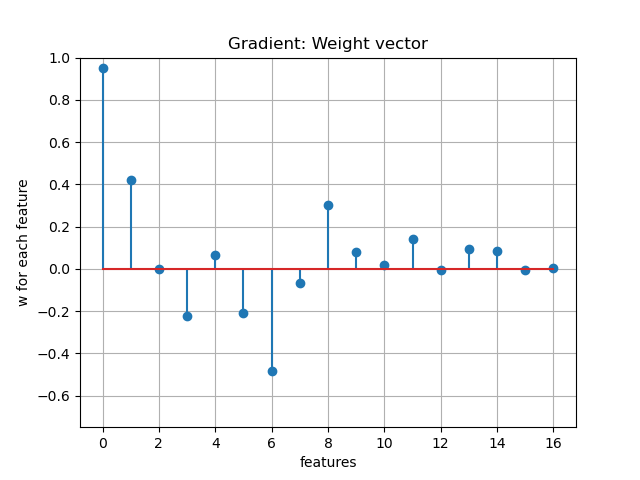
\includegraphics[width=.5\textwidth]{GradientWeightvector.PNG}}
			\subfloat[][\emph{$\hat {y} - y$ for Test and train}\label{fig:ga_b}]
			{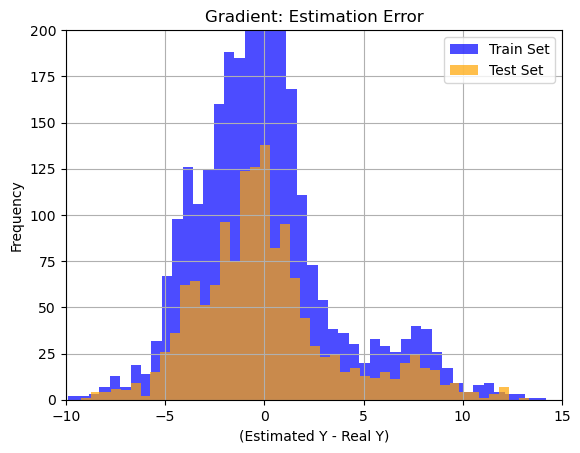
\includegraphics[width=.5\textwidth]{GradientEstimationError_test.PNG}}\\
			\subfloat[][\emph{$\hat { \mathbf { y } } _ { \mathrm { train } } \textit{{\scriptsize VS} }  \mathbf {y } _ { \mathrm { train } }$}\label{fig:ga_c}]
			{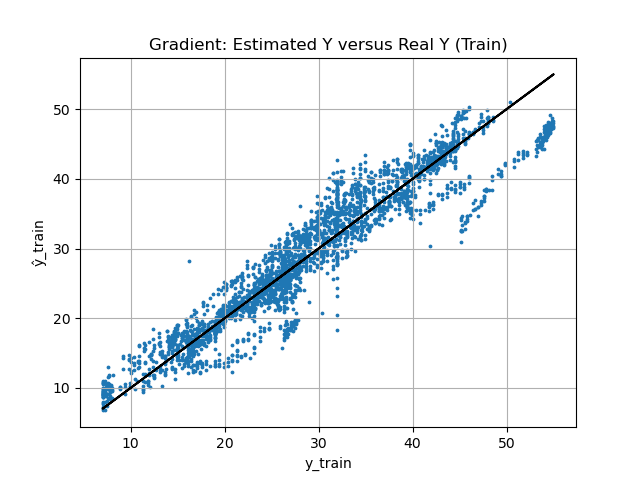
\includegraphics[width=.5\textwidth]{GradientEstimatedYversusRealY_train.PNG}}
			\subfloat[][\emph{$\hat { \mathbf { y } } _ { \mathrm { test } } \textit{{\scriptsize VS} }  \mathbf {y } _ { \mathrm { test } }$}\label{fig:ga_d}]
			{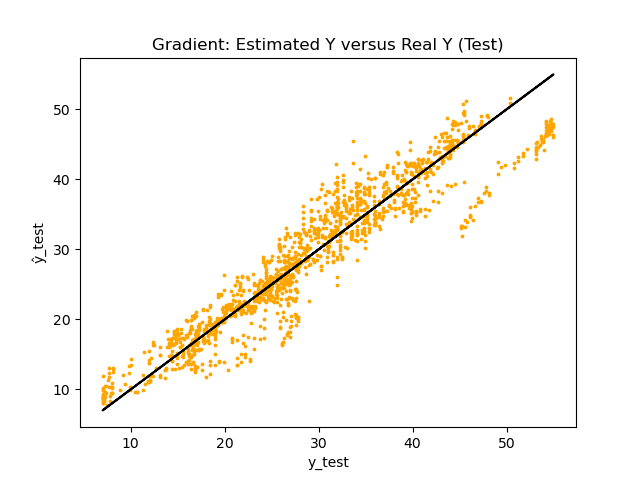
\includegraphics[width=.5\textwidth]{GradientEstimatedYversusRealY_test.PNG}}\\			
			\caption{The gradient algorithm}
			\label{fig:ga}
		\end{center}
	\end{figure}
			
	\subsection{The stochastic gradient}
	In the Stochastic Gradient we write the gradient of the cost function as
	\begin{equation}\label{2.8}
	\nabla f ( \mathbf { w } ) = \sum _ { n = 0 } ^ { N } \nabla f _ { n } ( \mathbf { w } ) = \sum _ { n = 0 } ^ { N } [ [ \mathbf { x } ( n ) ] ^ { T } \mathbf { w } - y ( n ) ] \mathbf { x } ( n )
	\end{equation}\\
	Starting from a random initial vector $w_{i}$, we find the next value of the vector as:
	\begin{equation}\label{2.9}
	\mathbf { w } _ { i + 1 } = \mathbf { w } _ { i } - \gamma \nabla f _ { i } ( \mathbf { w } _ { i } )
	\end{equation}
	\subsubsection{Result}
	Like previous sections, the figures \ref{fig:sg_a},\ref{fig:sg_b},\ref{fig:sg_c} and \ref{fig:sg_d} are representative of the good results given by the algorithm. By looking at figure \ref{fig:sg_a} it can be observed that also in this case feature 0 has most important weight over the other features (value of about 1).
	Points scattered in figures \ref{fig:sg_c} and \ref{fig:sg_d} this time seem a bit disperse.
	
	\begin{figure}[H]
		\centering
		\begin{center}
			\subfloat[][\emph{$w^*$ optimize vector}\label{fig:sg_a}]
			{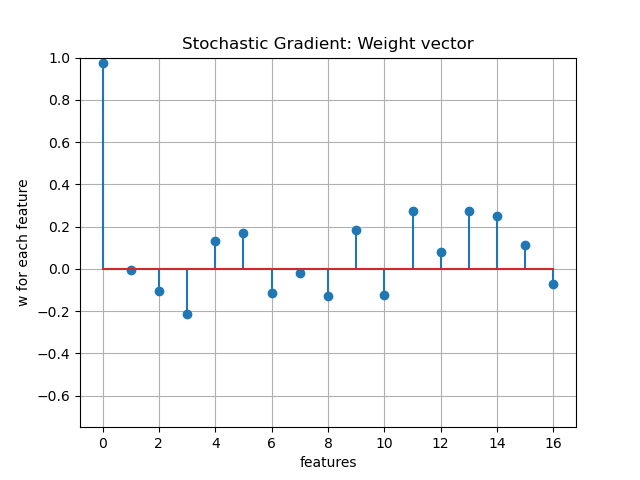
\includegraphics[width=.5\textwidth]{StochasticGradientWeightvector.PNG}}
			\subfloat[][\emph{$\hat {y} - y$ for Test and train}\label{fig:sg_b}]
			{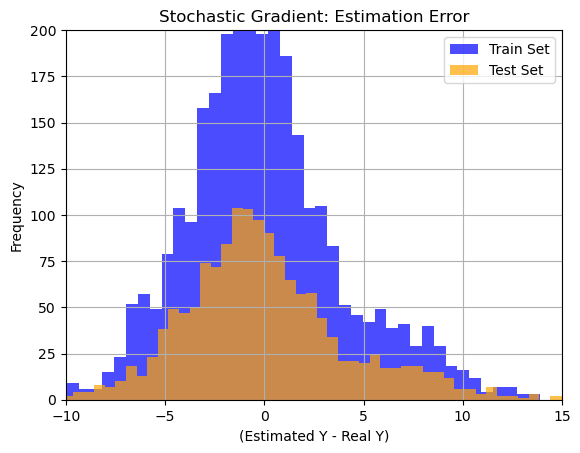
\includegraphics[width=.5\textwidth]{StochasticGradientEstimationError_test.PNG}}\\
			\subfloat[][\emph{$\hat { \mathbf { y } } _ { \mathrm { train } } \textit{{\scriptsize VS} }  \mathbf {y } _ { \mathrm { train } }$}\label{fig:sg_c}]
			{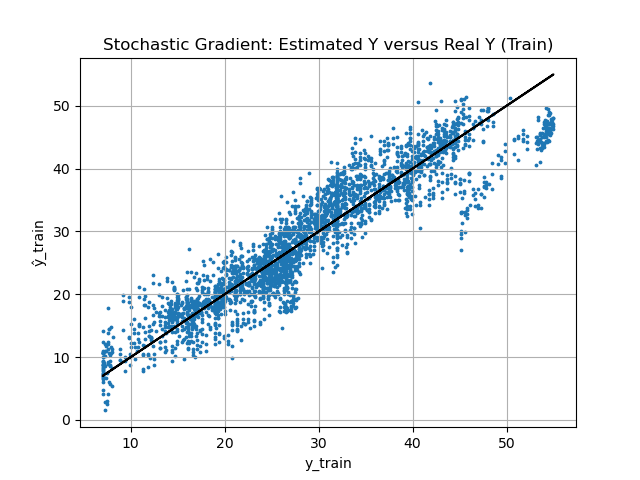
\includegraphics[width=.5\textwidth]{StochasticGradientEstimatedYversusRealY_train.PNG}}
			\subfloat[][\emph{$\hat { \mathbf { y } } _ { \mathrm { test } } \textit{{\scriptsize VS} }  \mathbf {y } _ { \mathrm { test } }$}\label{fig:sg_d}]
			{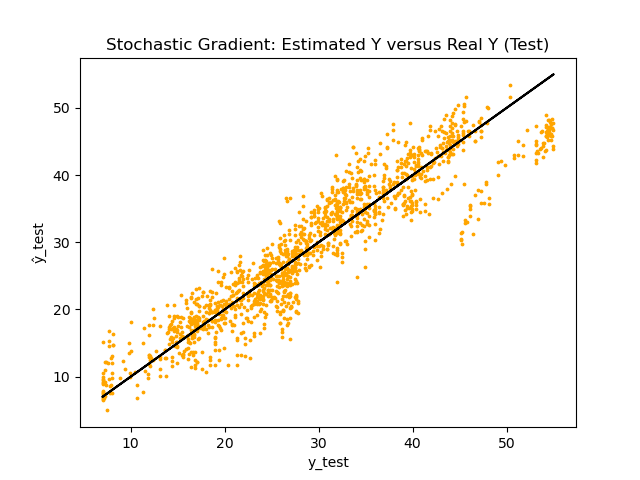
\includegraphics[width=.5\textwidth]{StochasticGradientEstimatedYversusRealY_test.PNG}}\\
			\caption{The stochastic gradient}
			\label{fig:sg}
		\end{center}
	\end{figure}
	
	
	\subsection{The conjugate gradient}
	Considering the Linear Least Square problem
	\begin{equation}
	f(w) = ||y-Xw||^2= \frac{1}{2} [y^Ty+w^TX^TXw-2y^TXw]
	\end{equation}
	in the \textbf{conjugate gradient} we assume
	\begin{equation}
	f(w) = \frac{1}{2} w^TX^TXw-y^TXw+\frac{1}{2} y^Ty =\frac{1}{2} Qw-b^Tw+c	
	\end{equation}
	where $Q=X^TX$ and $b= X^Ty$ and $c$ is constant that doesn't influence the value $W^*$. The gradient of $f(w^*)$ is:
	\begin{equation}
	\nabla f(w^*)=Qw^*-b=0
	\end{equation}
	A solution can be found with the help of \emph{conjugate vectors} which are vectors orthogonal with respect to a matrix $\vec{Q}$. It means that the vectors $\vec{d}_i$ and $\vec{d}_k$ are Q-orthogonal if $\vec{d}_i^T\vec{Q}\vec{d}_k=0$.	
	
	At first we set $\vec{d}_0=-\vec{g}_0=\vec{b}$ and $\vec{w}_0=0$ as the initial solution, where $\vec{g}$ is the direction of the gradient and $\vec{d}$ is the actual direction taken by the algorithm.
	The next directions are computed as $\vec{d}_{k+1}=-\vec{g}_{k+1}+\beta_{k}\vec{d}_k$ where $\beta$ is a coefficient that depends on the other parameters.
	
	\subsubsection{Result}
	Figure \ref{fig:sg_a} represents the feature with highest weight is again the first one, but the value is lower (0.5 instead of 0.95 as with the Gradient Algorithm and Steepest Descent). The other correlation of features are almost near 0.
	It can be noticed from figure \ref*{fig:sg_b} there is a wider distribution of error. The most of occurrences this time is almost around -0.3 and not exactly 0.  
	
	\begin{figure}[H]
		\centering
		\begin{center}
			\subfloat[][\emph{$w^*$ optimize vector}\label{fig:cg_a}]
			{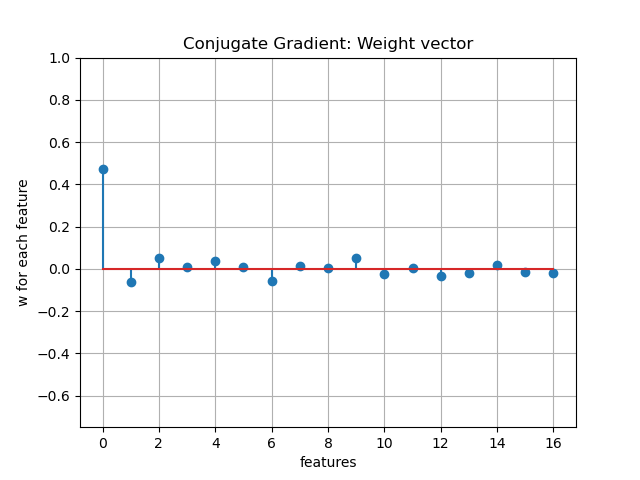
\includegraphics[width=.5\textwidth]{ConjugateGradientWeightvector.PNG}}
			\subfloat[][\emph{$\hat {y} - y$ for Test and train}\label{fig:cg_b}]
			{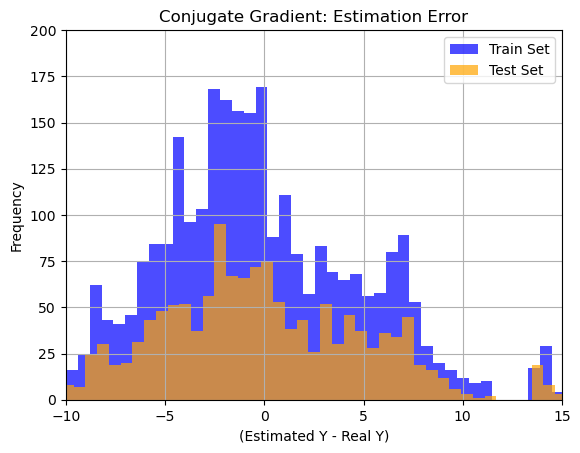
\includegraphics[width=.5\textwidth]{ConjugateGradientEstimationError_test.PNG}}\\
			\subfloat[][\emph{$\hat { \mathbf { y } } _ { \mathrm { train } } \textit{{\scriptsize VS} }  \mathbf {y } _ { \mathrm { train } }$}\label{fig:cg_c}]
			{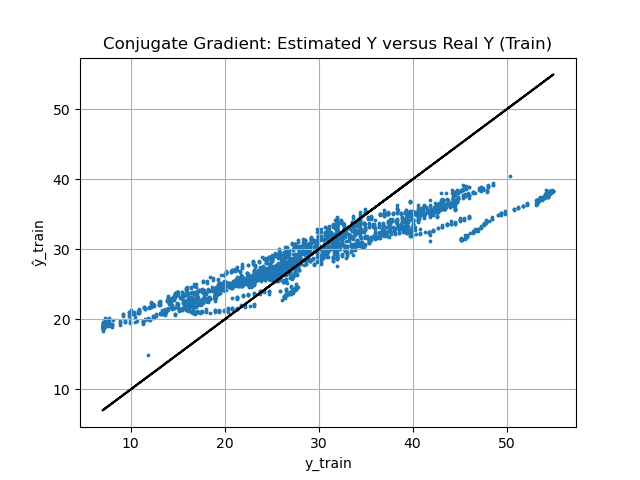
\includegraphics[width=.5\textwidth]{ConjugateGradientEstimatedYversusRealY_train.PNG}}
			\subfloat[][\emph{$\hat { \mathbf { y } } _ { \mathrm { test } } \textit{{\scriptsize VS} }  \mathbf {y } _ { \mathrm { test } }$}\label{fig:cg_d}]
			{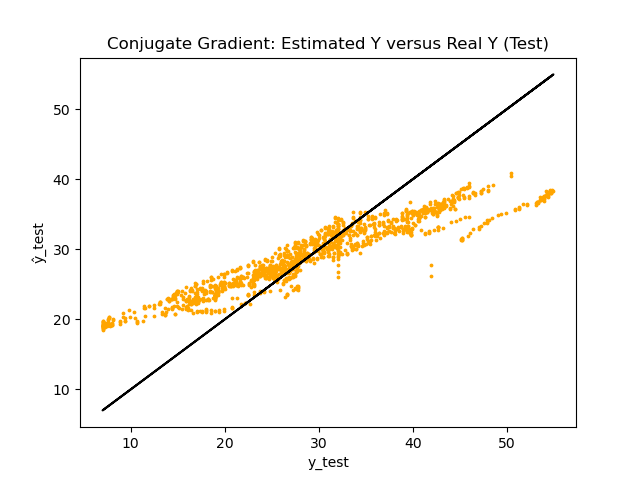
\includegraphics[width=.5\textwidth]{ConjugateGradientEstimatedYversusRealY_test.PNG}}\\
			\caption{The conjugate gradient}
			\label{fig:cg}
		\end{center}
	\end{figure}
	\subsection{The steepest descent algorithm}
	The steepest decent algorithm is used to optimize the step of the gradient algorithm. If $\gamma$ is very small, it would take long time to converge and become computationally expensive. If $\gamma$ is large, it may fail to converge and overshoot the minimum. Our goal is to find the optimum vector \textbf{w} and with this iterative method, we will improve step by step our $\gamma$ by evaluating, for each $\mathbf{x_i}$ the $\nabla f ( \mathbf { x_i } ) $ and the Hessian Matrix in that point: $\mathbf { H } \left( \mathbf { x } _ { i } \right) = 2 \mathbf { X } ^ { T } \mathbf { X }$.
	
	\begin{flushright}
		\begin{equation}
		\gamma _ { i } = \frac { \left\| \nabla f \left( \mathbf { x } _ { i } \right) \right\| ^ { 2 } } { \nabla f \left( \mathbf { x } _ { i } \right) ^ { T } \mathbf { H } \left( \mathbf { x } _ { i } \right) \nabla f \left( \mathbf { x } _ { i } \right) }
		\end{equation}\\
		
		
		\begin{equation}
		\mathbf { x } _ { i + 1 } = \mathbf { x } _ { i } - \gamma _ { i } \nabla f \left( \mathbf { x } _ { i } \right)
		\end{equation}
	\end{flushright}

	\subsubsection{Result}		
	As in the previous algorithms, in the figures \ref{fig:sda_c} and \ref{fig:sda_d} we see how well the algorithm performs and the method fits well the dataset. in figure \ref{fig:sda_a} it can seen correlation of features are almost like correlation of stochastic gradient algorithm. In histogram of figure \ref{fig:sda_b} we have again the highest value in feature 0.
 	\begin{figure}[H]
		\centering
		\begin{center}
			\subfloat[][\emph{$w^*$ optimize vector}\label{fig:sda_a}]
			{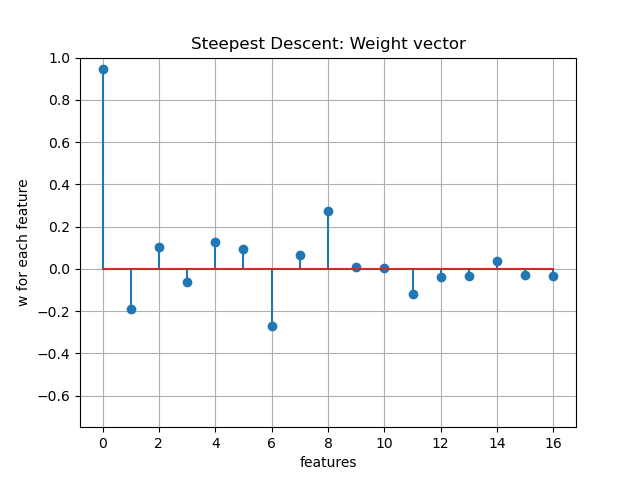
\includegraphics[width=.5\textwidth]{SteepestDescentWeightvector.PNG}}
			\subfloat[][\emph{$\hat {y} - y$ for Test and train}\label{fig:sda_b}]
			{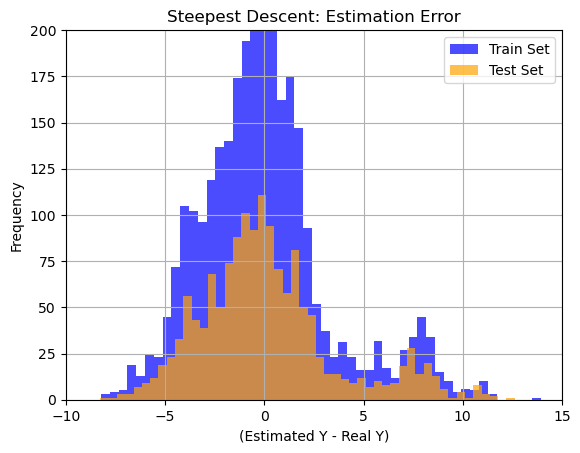
\includegraphics[width=.5\textwidth]{SteepestDescentEstimationError_test.PNG}}\\
			\subfloat[][\emph{$\hat { \mathbf { y } } _ { \mathrm { train } } \textit{{\scriptsize VS} }  \mathbf {y } _ { \mathrm { train } }$}\label{fig:sda_c}]
			{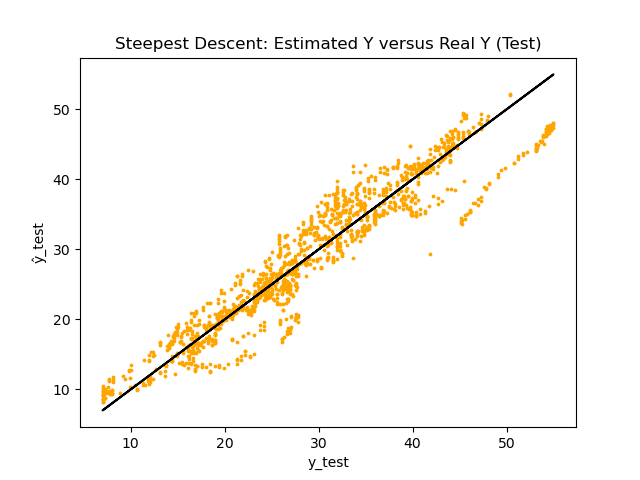
\includegraphics[width=.5\textwidth]{SteepestDescentEstimatedYversusRealY_test.PNG}}
			\subfloat[][\emph{$\hat { \mathbf { y } } _ { \mathrm { test } } \textit{{\scriptsize VS} }  \mathbf {y } _ { \mathrm { test } }$}\label{fig:sda_d}]
			{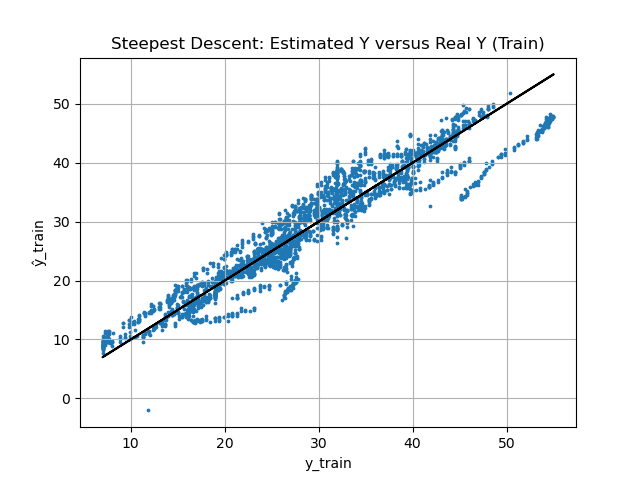
\includegraphics[width=.5\textwidth]{SteepestDescentEstimatedYversusRealY_train.PNG}}\\
			\caption{The steepest descent algorithm}
			\label{fig:sda}
		\end{center}
	\end{figure}
	
	\newpage
	\subsection{The ridge regression (optimize $\lambda$)}
	It is possible that vector $w^*$ takes very large values and over-fitting occurs, due to this reason, it might be convenient to solve the new problem:
	
	\begin{equation}
	\operatorname { min } _ { \mathbf { w } } \| \mathbf { y } - \mathbf { X } \mathbf { w } \| ^ { 2 } + \lambda \| \mathbf { w } \| ^ { 2 } = \operatorname { min } _ { \mathbf { w } } f ( \mathbf { w } )
	\end{equation}\\
	where $\lambda$ has to be set conveniently (trial and error). The solution of this problem can then be obtained using the pseudo-inverse
	
	\begin{equation}
	\nabla f ( \mathbf { w } ) = 2 \mathbf { X } ^ { \top } \mathbf { X } \mathbf { w } - 2 \mathbf { X } ^ { \top } \mathbf { y } + 2 \lambda \mathbf { w } = 0
	\end{equation}
	so we get	
	\begin{equation}
	\hat { \mathbf { w } } = \left( \mathbf { X } ^ { \top } \mathbf { X } + \lambda \mathbf { I } \right) ^ { - 1 } \mathbf { X } ^ { \top } \mathbf { y }
	\end{equation}
	
	\subsubsection{Result}
	Looking at Figures \ref{fig:rr_c} and \ref{fig:rr_d} it can be easily noticed that those figures are very similar to the ones of Gradient and Steepest Descent Algorithms: large bandwidth (from about -0.7 to 1.1) and not symmetric shapes; of course, also the distributions of points in figure \ref{fig:rr_b} are pretty much the same to those in the same algorithm named before.
	\begin{figure}[H]
		\centering
		\begin{center}
			\subfloat[][\emph{$w^*$ optimize vector}\label{fig:rr_a}]
			{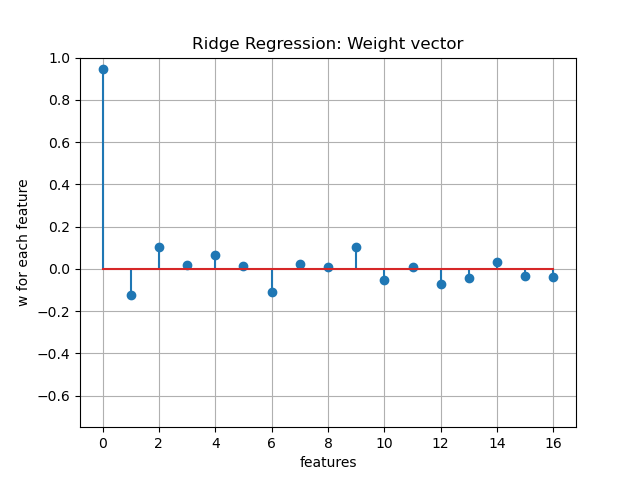
\includegraphics[width=.5\textwidth]{RidgeRegressionWeightvector.PNG}}
			\subfloat[][\emph{$\hat {y} - y$ for Test and train}\label{fig:rr_b}]
			{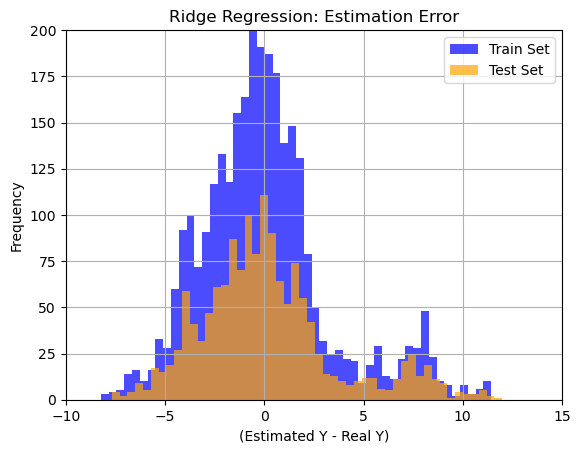
\includegraphics[width=.5\textwidth]{RidgeRegressionEstimationError_test.PNG}}\\
			\subfloat[][\emph{$\hat { \mathbf { y } } _ { \mathrm { train } } \textit{{\scriptsize VS} }  \mathbf {y } _ { \mathrm { train } }$}\label{fig:rr_c}]
			{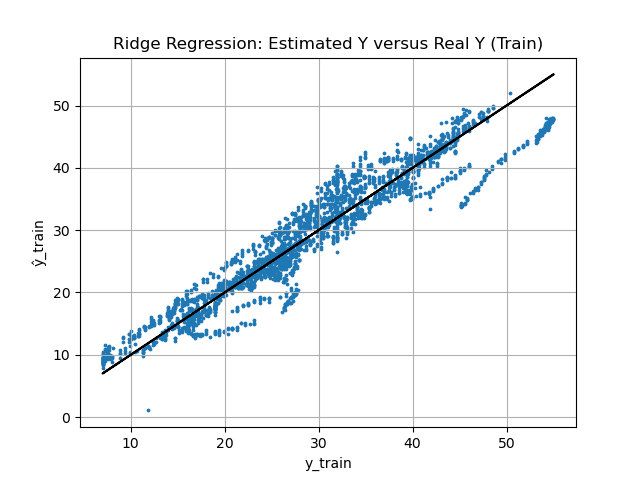
\includegraphics[width=.5\textwidth]{RidgeRegressionEstimatedYversusRealY_train.PNG}}
			\subfloat[][\emph{$\hat { \mathbf { y } } _ { \mathrm { test } } \textit{{\scriptsize VS} }  \mathbf {y } _ { \mathrm { test } }$}\label{fig:rr_d}]
			{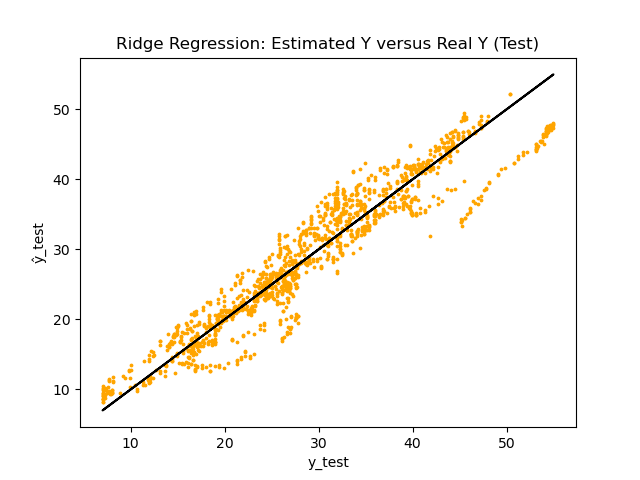
\includegraphics[width=.5\textwidth]{RidgeRegressionEstimatedYversusRealY_test.PNG}}\\
			\caption{The ridge regression (optimize $\lambda$)}
			\label{fig:rr}
		\end{center}
	\end{figure}
	
	\section{Conclusions}
	 Comparing the results from all the algorithms in terms of Mean Square Error which shown in figure \ref{fig:err}, more or less all the algorithms return similar Mean Square Error, this means that we can use each of them in the same way.
	 \begin{figure}[H]
	 	\centering
	 	\begin{center}
	 		\subfloat[][\emph{the gradient algorithm}\label{fig:rr_a}]
	 		{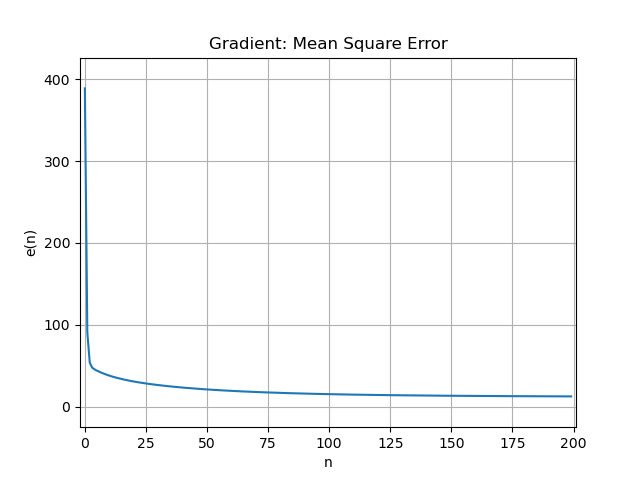
\includegraphics[width=.5\textwidth]{GradientMeanSquareError.PNG}}
	 		\subfloat[][\emph{the stochastic gradient}\label{fig:rr_b}]
	 		{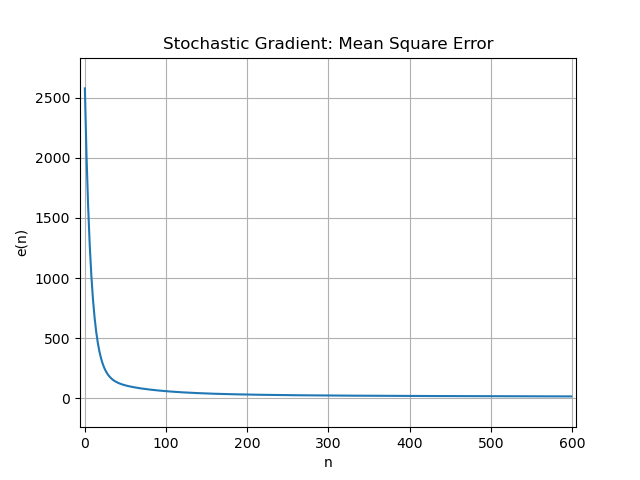
\includegraphics[width=.5\textwidth]{StochasticGradientMeanSquareError.PNG}}\\
	 		\subfloat[][\emph{the conjugate gradient}\label{fig:rr_c}]
	 		{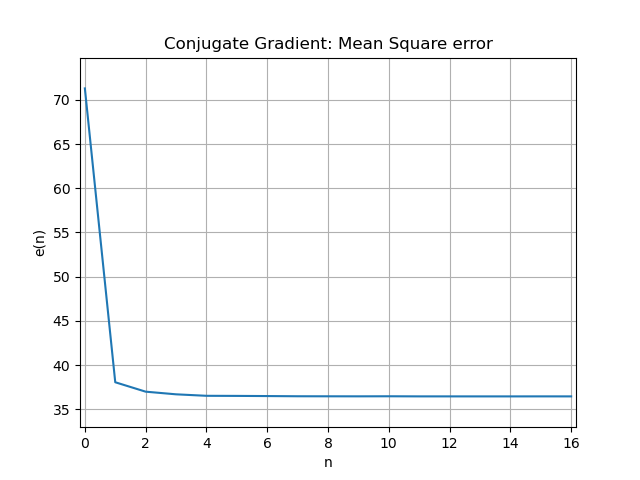
\includegraphics[width=.5\textwidth]{ConjugateGradientMeanSquareerror.PNG}}
	 		\subfloat[][\emph{the steepest descent algorithm}\label{fig:rr_d}]
	 		{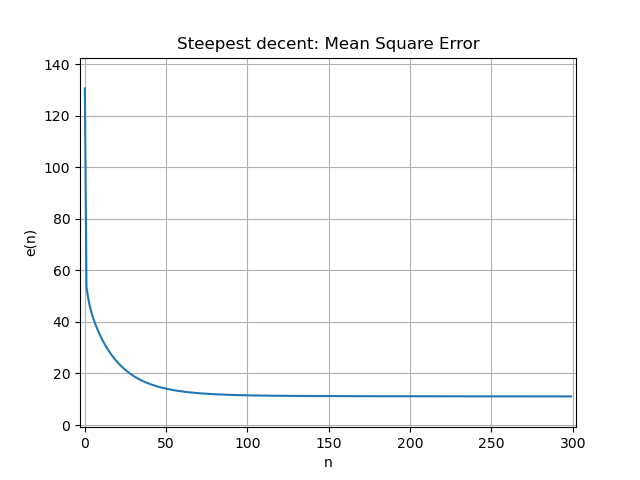
\includegraphics[width=.5\textwidth]{SteepestdecentMeanSquareError.PNG}}\\
	 		\subfloat[][\emph{the ridge regression}\label{fig:rr_d}]
	 		{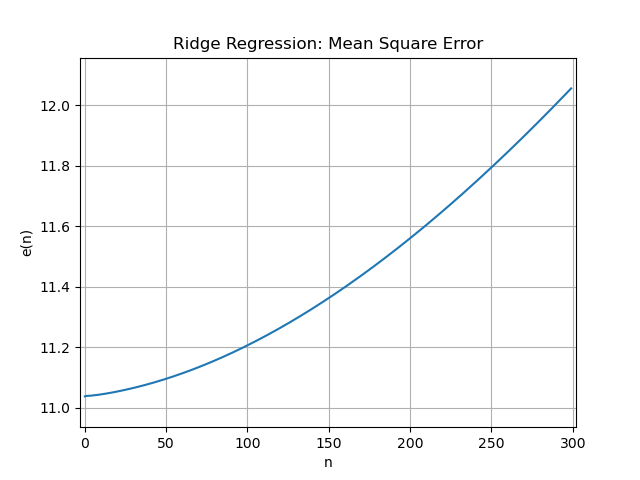
\includegraphics[width=.5\textwidth]{RidgeRegressionMeanSquareError.PNG}}\\
	 		\caption{\textbf{Mean square error of algorithms}}
	 		\label{fig:err}
	 	\end{center}
	 \end{figure}
	
	
	
\end{document}